% !TEX root = CI_Adoption.tex

\section{Results and Discussion}
\label{sec:results}
We discuss changes in development practices after CI adoption along four 
dimensions: code churn, commit frequency, issue tracking, and testing. 

\subsection{Preliminaries}
\label{sec:examples}

Before diving into quantitative analysis we eyeballed several projects in our 
collection. 
We observed that on several occasions \Tvis has been adopted as part of a 
larger scale restructuring effort. 
For instance, \texttt{allendevco/pill-logger} has started using \Tvis on November 
20, 2013; in the same period developers have changed the project build system 
from Ant to Gradle and, as a consequence of that, also changed the way the 
project folders are organized.
Similarly, \texttt{Netflix/denominator} has introduced \Tvis on March 13, 2015
after an active development period of daily commits starting on March 3.
On the very same date \Tvis has been introduced, the project updated library 
dependencies and restructured tests, while on the next day it added examples 
and removed support of DiscoveryDNS.
This rather active development continued until the version 4.5.0 has been 
released on April 6, 2015.
The project had three additional commits in April and then went to a recess 
until early August. 
Examples such as \texttt{allendevco/pill-logger} and \texttt{Netflix/denominator} 
suggest that the activity immediately prior and immediately after introduction 
of \Tvis might not be representative for the project's overall software development
practices.
Therefore, to limit the risk of our trends being biased by extraordinary project 
activity during the transition period, we decided to exclude one month before 
the first \Tvis build and one month after it, in our quantitative analyses below.

\begin{figure}[t]
\centering
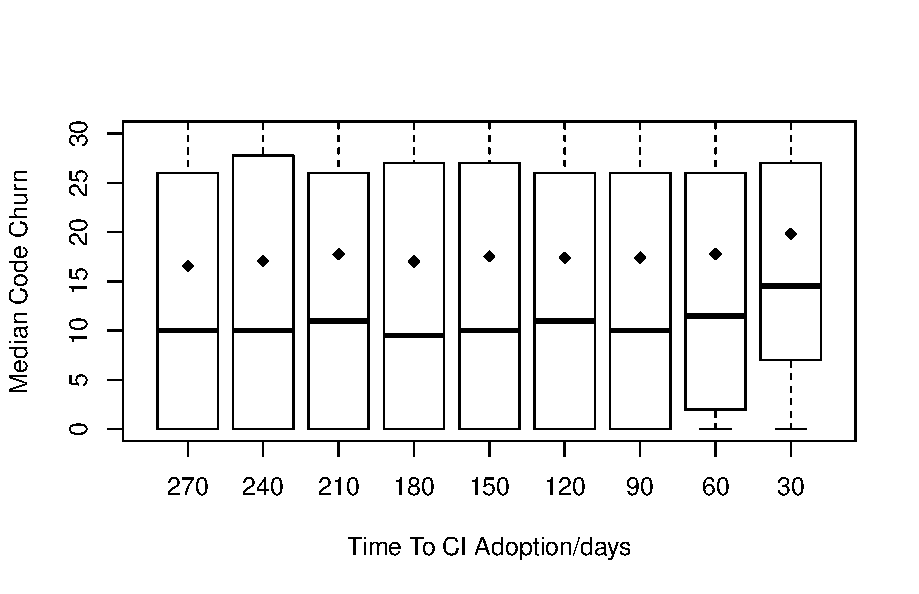
\includegraphics[width=0.45\textwidth, clip=true, trim=0 15 15 50]{churn_before.pdf}
\caption{Code churn before \Tvis adoption.}
\label{Fig:CodeChurnBefore}
\end{figure}


\begin{figure}[t]
\centering
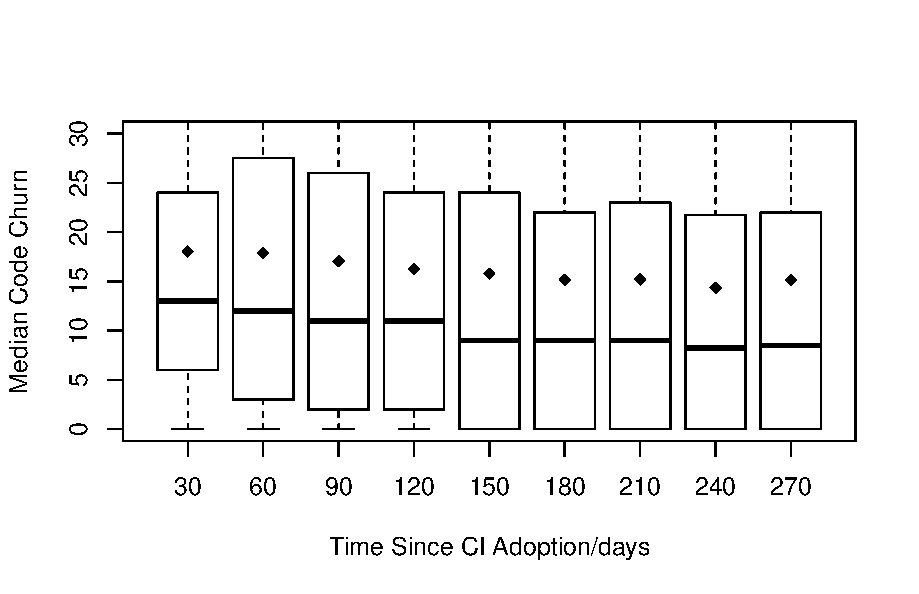
\includegraphics[width=0.45\textwidth, clip=true, trim=0 15 15 50]{churn_after.pdf}
\caption{Code churn after \Tvis adoption.}
\label{Fig:CodeChurnAfter}
\end{figure}


\subsection{RQ1: Trends in Code Churn}

The first development practice we examine is code churn.
Recall that our data consists of 567 projects, each with at least 500 non-merge 
commits.

\smallskip\noindent \emph{Exploratory Study}: To explore general trends over 
time, we first look at code churn in months leading up to CI adoption.
Fig.~\ref{Fig:CodeChurnBefore} shows a boxplot of per-project median code 
churn for each of nine consecutive 30-day time intervals before CI adoption.
The horizontal line in each boxplot is the median value of all per-project medians, 
and the black dot is their average value.
We observe that, for most part, the medians dance around 10 and 12 lines of 
code churn per period, and the averages between 16 and 18 lines, with large 
variance and no obvious trend. 
The 30-day interval just before CI adoption seems to stand out and is higher 
than the rest.

Next, we look to the other side of the adoption point. 
Fig.~\ref{Fig:CodeChurnAfter} shows a boxplot of per-project median code 
churn for each of nine consecutive 30-day time intervals following CI adoption.
Here, there seems to be a slight downward trend in both the medians and 
averages; the former drop monotonically from 13 down to 8 lines of code and 
the latter down to 15 lines of code.
However, we note the large variance around the medians.

The 30- and 60-day intervals just after the adoption point seem to be higher 
than the rest, and together with the 30-day interval just before adoption of CI 
seem to form a peak of increased code churn.
In conclusion, discounting the peak behavior in code churn around CI adoption 
time, we observe a small reduction in the amounts of code churn from before 
to after CI adoption.

% !TEX root = ../CI_Adoption.tex

\begin{table}[t] \centering
\small
  \caption{Model Coefficients for 566 Models of Code Churn}
  \label{Table:rddmodels}
\begin{tabular}{ l  r r r r }        
\hline 

 & $\beta$ & $\gamma$ & $\delta$ & $\beta + \delta$ \\ 
 \hline 
 \hline
not signif. & 504 & 508 & 514 & \\
\hline
signif., $>0$ & 45 & 28 & 10 & 13 \\
\hline
signif., $<0$ & 17 & 30 & 42 & 39 \\
\hline
\end{tabular}
\end{table}

\smallskip\noindent \emph{Statistical Modeling Study}: 
Guided by our observations from the exploratory study above, we proceed to 
quantify the trends we observed.
For each project, we fitted a sharp RDD model, as described before.
Recall that because of the peak we observed, we eliminated the time point 
immediately before and the one immediately after the CI adoption time, so as 
they do not throw off the regression models.
Table~\ref{Table:rddmodels} summarizes the results for the models on the 
remaining 16 time points.
Recall that $\beta$ is the slope before, $\gamma$ the size of the effect of 
CI introduction, $\delta$ is the divergence in the slopes before and after CI 
adoption, and $\beta + \delta$ the slope of the linear trend after CI adoption.

Of the 567 models, in 487 there was no significant linear relationship of 
code churn to time, \ie there was no linear trend.
In 47 projects there was a rising trend before CI and in 33 projects a falling 
trend before CI.
Similarly, in 507 projects no effect of CI introduction on code churn was found. 
Among the 58 projects where an effect was significant, in 34 the trend was 
positive, \ie code churn increased, and in 24 it was negative, \ie code churn 
decreased.
Interestingly, while in 487 projects no change of slope in the trends before 
and after CI adoption was found, in the 80 projects with significant change 
of trends, a reduction in the slope was more prevalent than an increase by 
about 2 to 1.
This carried over into trends following CI adoption: out of the 80 significant 
trend changes, 55 are downward trends, and only 25 are upward.


%Table XX: Projects with statistical negative trends after CI

\smallskip\noindent \emph{Discussion}:
Most of the projects did not show linear trends with time in code churn, on 
either side of the CI adoption time.
One explanation consistent with this is that any phenomena giving rise to 
pressures to increase or reduce code churn are not long term/sustained or, 
alternatively, perhaps they are subordinate in magnitude to other, more 
pressing phenomena of local character in time.
It is also likely that our models and data are insufficient to capture them.
Some of the reasons for this are: low temporal resolution, high dispersion 
of the data, non-uniform distribution of the events across time, and project 
specific considerations that we could not model.

Our exploratory study showed a peak around CI adoption time and a slight 
downward trend following CI adoption.
The modeling study showed that when linear trends were present (in 15\% 
of the models), the downward one after CI adoption were twice as frequent 
as the upward one, a reversal of the pattern in the trends from before CI.
This is consistent with Fowler's recommended good practices of CI, of 
committing smaller changes to the code.
Alternatively, it is also consistent with the observation by Brindescu 
\etal~\cite{brindescu2014centralized} that, as projects age, bug-fixing 
commits, which on average are smaller, become more prevalent than 
commits adding new features, which on average are larger.

The models also showed that when present, the effect of CI adoption on the 
amount of code churn right after was positive in more cases than negative.
The increased code churn on both sides near the CI adoption time is 
arguably in line with expectations that more maintenance work may be 
going on in preparation for the transition to CI, and that the projects go 
through some adjustment/cleanup period right after.


\subsection{RQ2: Trends in Commit Frequency}

The second development practice we examine is commit frequency.
We use the same data as before, 567 projects, each with at least 500 
non-merge commits.

\begin{figure}[!t]
\centering
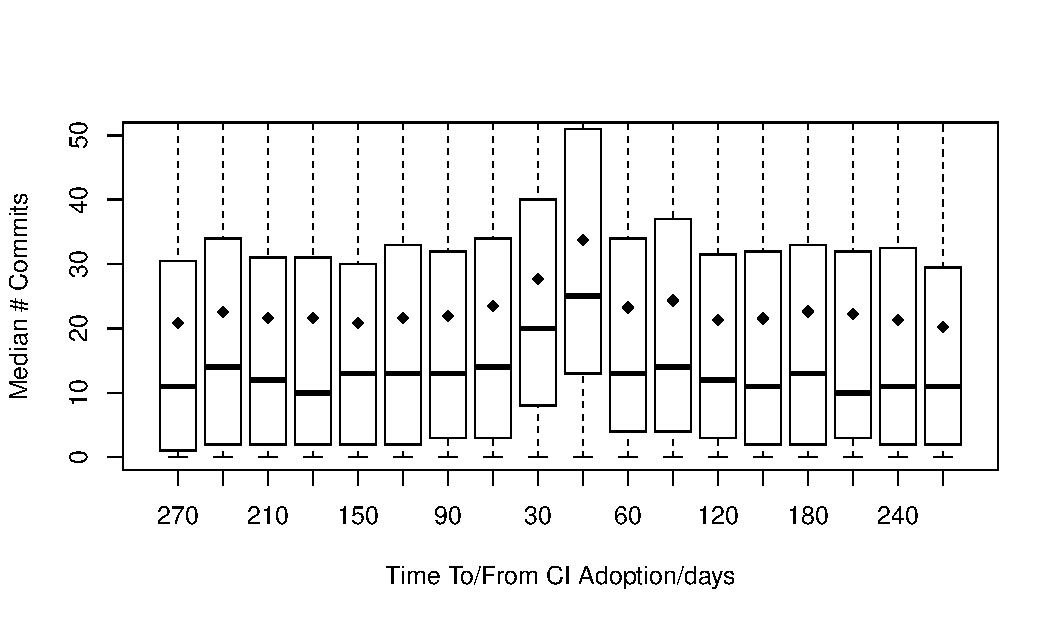
\includegraphics[width=0.45\textwidth, clip=true, trim=0 15 15 50]{numbercommits.pdf}
\caption{Commit frequency before and after CI adoption}
\label{Fig:NumberCommits}
\end{figure}

\smallskip\noindent \emph{Exploratory Study}: 
To explore general trends over time, we first look at commit frequency in 
the months leading up to CI adoption.
Figs.~\ref{Fig:NumberCommits} shows the boxplots of per-project median 
number of commits for each of nine consecutive 30-day time intervals 
before CI adoption and, respectively, nine consecutive 30-day time intervals 
after CI adoption.
As before, the horizontal line in each boxplot is the median value of all 
per-project medians, and the black dot is their average value.

As was the case with code churn, here we also see a peak in the 30-day 
interval just before and the one just after CI adoption.
Unlike for code churn, here we do not observe an apparent trend in the 
median or average commit frequency.

\smallskip\noindent \emph{Statistical Modeling Study}: 
As in RQ1, we fitted a sharp RDD model for each project, as described before.
Table~\ref{Table:rddmodels_freq} summarizes the results.
Recall that we eliminated one time point on either side of the CI adoption 
time so as they do not throw off the regression models.
% !TEX root = ../CI_Adoption.tex

\begin{table}[t] \centering
\small
  \caption{Model Coefficients for 567 Models of Commit Frequency}
  \label{Table:rddmodels_freq}
\begin{tabular}{ l  r r r r }        
\hline 

 & $\beta$ & $\gamma$ & $\delta$ & $\beta + \delta$ \\ 
 \hline 
 \hline
not signif. & 452 & 466 & 454 & \\
\hline
signif., $\ge 0$ & 71 & 59 & 33 & 42 \\
\hline
signif., $<0$ & 44 & 42 & 80 & 71 \\
\hline
\end{tabular}
\end{table}

\begin{table}[t] \centering
\small
  \caption{Model Coefficients for 370 Models of Merge Commit Frequency}
  \label{Table:rddmodels_merge_freq}
\begin{tabular}{ l  r r r r }        
\hline 

 & $\beta$ & $\gamma$ & $\delta$ & $\beta + \delta$ \\ 
 \hline 
 \hline
not signif. & 296 & 307 & 301 & \\
\hline
signif., $\ge 0$ & 46 & 35 & 26 & 44 \\
\hline
signif., $<0$ & 28 & 28 & 43 & 30 \\
\hline
\end{tabular}
\end{table}

In 452 (80\%) of the models, there was no significant linear relationship 
between commit frequency and time, \ie there was no linear trend.
In 71 projects there was a rising trend in commit frequency before CI 
and in 44 projects a falling trend before CI.
Similarly, in 466 projects no effect of CI introduction on commit frequency 
was found. 
Among the 101 projects where an effect was significant, in 59 the trend 
was positive, \ie commit frequency increased, and in the rest it was 
negative, \ie commit frequency decreased.
The mean value over all projects for $\gamma$, the effect size of CI 
adoption, was $1.1$ commit.
While in 454 projects no change of slope in the trends before and after CI 
adoption was found, in the 113 with significant change of trends a reduction 
in the slope was more prevalent than an increase by about 2.5 to 1.
This carried over to a lesser degree into trends in commit frequency 
following CI adoption: out of the 113 significant trend changes, 71 are 
downward trends, and 42 are upward.

\smallskip\noindent \emph{Discussion}:
As was the case for  code churn, most of the projects did not have longitudinal linear trends, for reasons probably similar to those 
in case of the code churn.

While our exploratory study did not suggest presence of a trend, the 
modeling study suggests that right after CI adoption there is a slight 
positive effect (after removing the peak months around CI adoption time). 
However, this effect is not sustained if a linear trend is present, which is 
2.5 times as likely to be decreasing as increasing. 
Given the expected increase in the frequency of commits expressed and 
encouraged by Fowler, this result might appear surprising.
It is possible that some saturation to the commit frequency has already 
been reached even before the CI adoption time.
As we see next, it is also likely developers are spending more time on 
automated testing.


%\as{Vladimir, do you have a cross-combination data, such as \# decrease in churn AND increase in frequency?}



\subsection{RQ3: Trends in Issue Report Frequency}

The third development practice we examine is issue report frequency.
As described above, we use data on 293 projects, each with at least 
100 issues.

\begin{figure}[t]
\centering
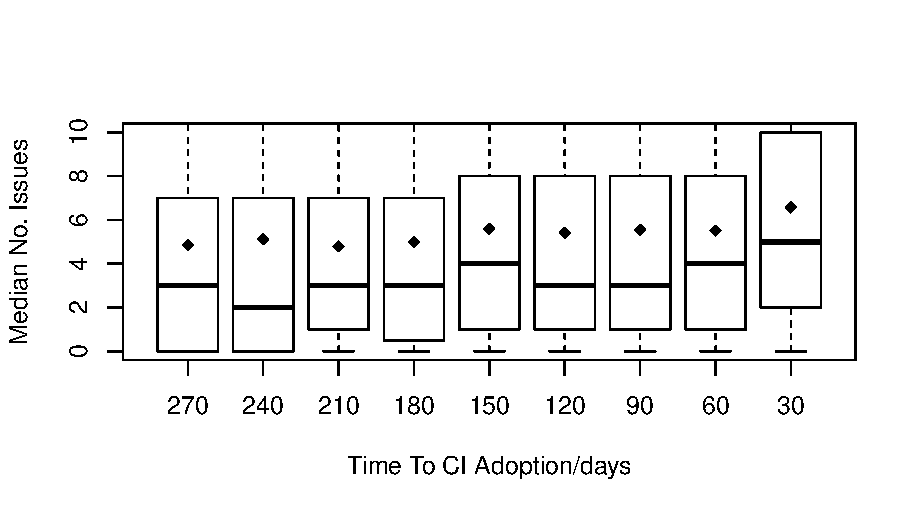
\includegraphics[width=0.45\textwidth, clip=true, trim=0 15 15 50]{issues_before.pdf}
\caption{Median number of issues before CI adoption}
\label{Fig:IssuesBefore}
\end{figure}


\begin{figure}[t]
\centering
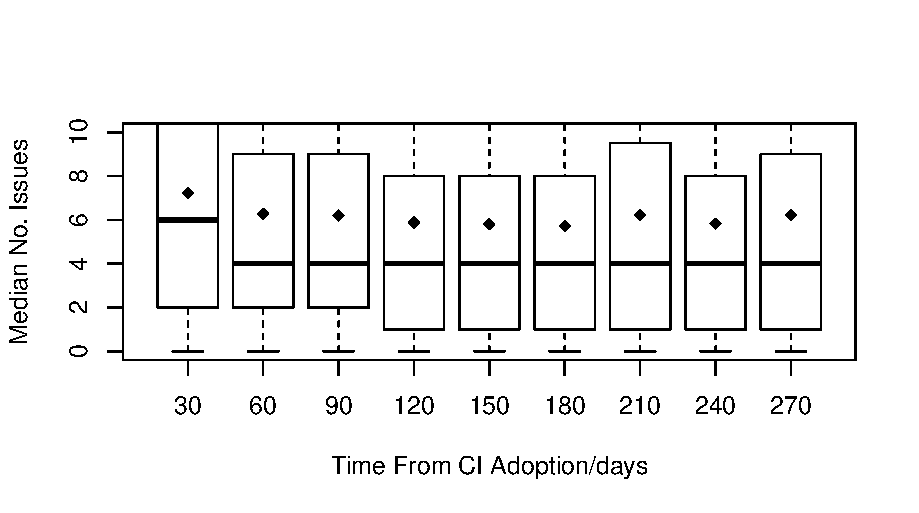
\includegraphics[width=0.45\textwidth, clip=true, trim=0 15 15 50]{issues_after.pdf}
\caption{Median number of issues after CI adoption}
\label{Fig:IssuesAfter}
\end{figure}

\smallskip\noindent \emph{Exploratory Study}:
We follow the same approach as in RQ1 and RQ2 and compare the 
medians and the averages in the number of issues per time period, in the 
months before and after the adoption of CI.
Fig.~\ref{Fig:IssuesBefore} and \ref{Fig:IssuesAfter} plot the number of 
issues per unit time period.
Observing these figures we can see that the months immediately preceding 
and following the adoption of CI exhibit the highest number of issues.
Following the adoption of CI the median of the number of issues seems to 
stabilize, while averages do not show a clear trend. 

% !TEX root = ../CI_Adoption.tex

\begin{table}[t] \centering
\small
  \caption{Model Coefficients for 291 Models of Issues Frequency}
  \label{Table:rddmodels_freq}
\begin{tabular}{ l  r r r r }        
\hline 

 & $\beta$ & $\gamma$ & $\delta$ & $\beta + \delta$ \\ 
 \hline 
 \hline
not signif. & 230 & 254 & 242 & \\
\hline
signif., $>0$ & 43 & 26 & 14 & 15 \\
\hline
signif., $<0$ & 18 & 11 & 35 & 33 \\
\hline
\end{tabular}
\end{table}

\smallskip\noindent \emph{Modeling Study}:
Results of the RDD modeling are summarized in Table~\ref{Table:rddmodels_issues}.
The lower number of projects in Table~\ref{Table:rddmodels_issues} 
compared to Tables~\ref{Table:rddmodels} and~\ref{Table:rddmodels_freq} 
should not be surprising. 
Recall from Section~\ref{sec:dd} that to answer RQ3 we have focused on 
projects having at least 100 issues, further reducing the size of the data set 
used in RQ1 and RQ2 to 293.
We have fitted models to 291 projects of the 293, however in most cases we 
did not observe linear trends.
When a linear trend has been observed than it was more than twice more 
often decreasing than increasing.
The mean value over all projects for $\gamma$, the effect size of CI adoption, 
was $1.0$ issue.


\smallskip\noindent \emph{Discussion}:

Again, most of the projects did not have longitudinal linear trends for reasons probably similar to those 
in the case of the code churn.


 Thus, we conclude the effect of CI adoption led to an overall increase of one 
 issue more per period.\vf{This needs text}




\subsection{RQ4: Trends in Testing}

The last development practice we examine is testing and the evolution 
of the types of errors revealed by automated testing.
The data consists of 250 projects, each with at least 100 builds, and 90\% 
of builds executing tests.

\begin{figure}[!t]
\centering
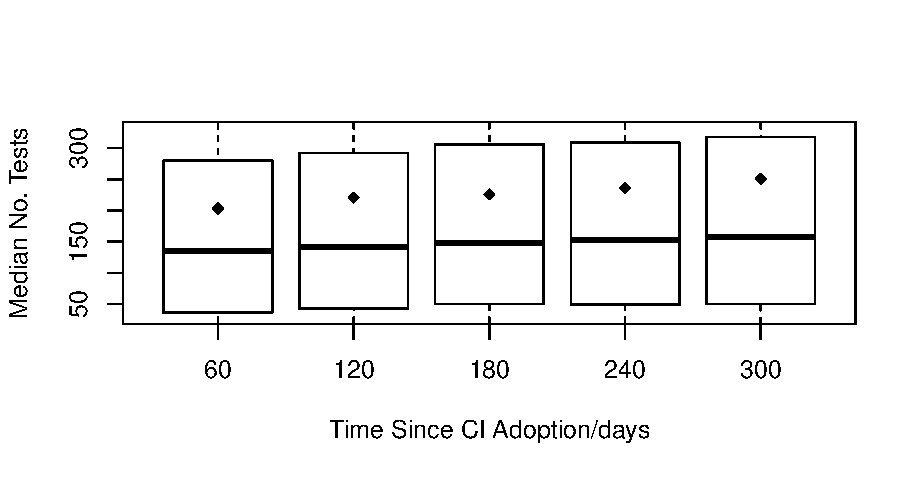
\includegraphics[width=0.45\textwidth, clip=true, trim=0 15 15 50]{tests.pdf}
\caption{Unit tests per build following CI adoption}
\label{Fig:Tests}
\end{figure}

\smallskip\noindent \emph{Exploratory Study}: 
As before, we first look for general trends over time.
Fig.~\ref{Fig:Tests} shows a boxplot of per-project median number of tests 
per build, for each of five consecutive 60-day time intervals before CI adoption.
We aggregated the data here in 60 day intervals to make it easier to visualize 
the trend, since the differences are small.
The horizontal line in each boxplot is the median value of all per-project medians, 
and the black dot is their average value.
We observe a monotonically increasing trend in both the medians, from 140 to 
160 tests per build, and the means, from 205 to 245 tests per build, \ie 15\% to 
20\% increase. 

To ascertain if the complexity of builds increases over time, we also calculated 
the average number of jobs per build.
The median is $1$ for all five time intervals.
These two findings suggest strongly that there is an increase in the number of 
unit tests per build over time.
This, coupled with our finding that builds are not getting more complex over time indicates that developers are likely spending more time on 
automated testing since CI adoption.
This is consistent with Fowler's "good practices" proposal.



\smallskip\noindent \emph{Error Types Study}:
We also looked at the evolution of the error types in builds over time after CI 
adoption.
For all 250 projects above, we looked at the builds that resulted in errors, 
and deconvolved the errors into 8 types, as described above.
We did this over 3 intervals: 0-60 days, 61-180 days, and 181-300 days (\ie 
corresponding to the first, third, and fifth interval in Fig.~\ref{Fig:Tests}).
The results are shown in Fig.~\ref{Fig:BugTypes}, where on the y-axis are 
the proportion of all erroneous builds that yield that error type.
We find an apparent upward trend over time in most error type categories, 
most notably compile errors, execution errors, failed tests, and skipped 
test.\footnote{The median number of error types per build remained $2$ over 
time.}
All these are consistent with an increase in the amount of code being built 
and tested per build, as well as an increasing management of errors by 
skipping tests, likely to aid in debugging.
On the other hand, we find a decreasing trend among errors related to missing 
files/dependencies, and time-outs, both consistent with those errors being less 
of an issue over time, as developers are acculturating to the CI mediated 
processes.

Thus, overall we find an expected adjustment to the automated testing and 
error handling, with an indication that debugging complexity grows over time.

%%this is the old plots
%\begin{figure}[!t]
%\centering
%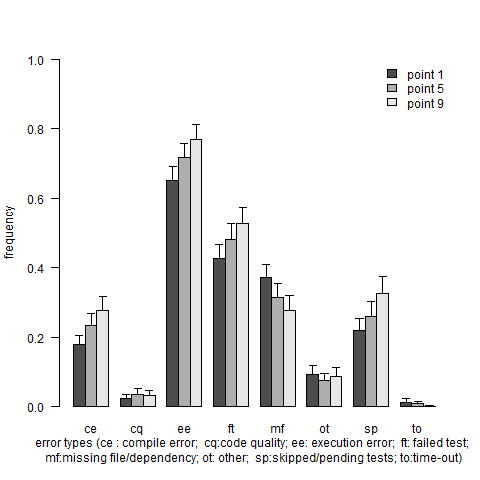
\includegraphics[width=0.45\textwidth, clip=true, trim=0 15 15 50]{plot_together.png}
%\caption{Evolution of Error Types Since CI Adoption}
%\label{Fig:BugTypesold}
%\end{figure}


%this is the new plots
\begin{figure}[!t]
	\centering
	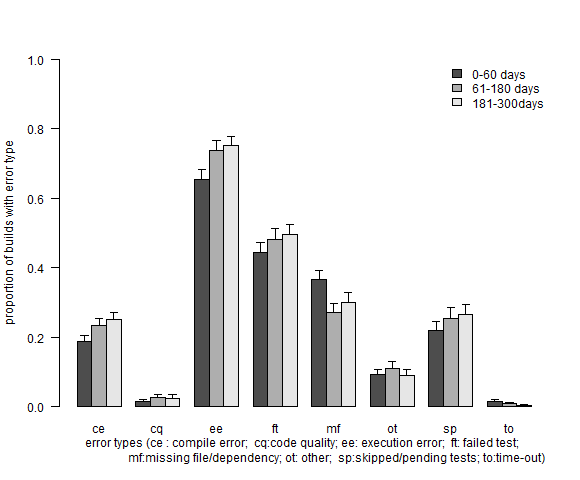
\includegraphics[width=0.45\textwidth, clip=true, trim=0 15 15 50]{new_plot_together.png}
	\caption{Evolution of Error Types Since CI Adoption}
	\label{Fig:BugTypes}
\end{figure}

